\chapter{Methodology}
\label{ch:Methodology}
% Most important chapter: talks about my contribution to the topic and what I have achieved

% Goal: Detect ambiguous words in a sentence without context
% 	- Develop method(s) to differentiate from non-ambiguous words: uncover patterns in translation and backtranslation
% 	- Finetune parameters (e.g. how often ambiguous word reoccurs in backtranslation; how many unique words in translation vs. backtranslation)
% 	(-) Suggest alternative translations to ambiguous word
%   (-) Differentiate ambiguous from biased words (cannot say if bias exists or not -> Quality Estimation)

In this chapter, I present the methods used for detecting ambiguity in MT. First, I define the problem around ambiguity that this study attempts to solve. Then, I outline the systematic approach used to solve the problem at hand.

%%%%%%%%%%%%%%%%%%%%%%%%%%%%%%%%%%%%%%%%%%%%%%%%%%%%%%%%%%%%%%%%%%%%%%%%%%%%%%%%%%%%%%%%%%%%
\section{Problem Statement}
\label{sec:Methodology:Problem}

It has been proven that NMT systems reinforce bias present in the training data (e.g., \citet{Prates_2019}, \citet{Stanovsky_2019}). This is typically the case when translating from genderless or notional languages (e.g., English) into grammatical gender languages (e.g., German, Spanish, Russian). One of the most common type of bias is gender bias. 
This bias is often reflected in the way NMT systems translate occupations, since many professions are stereotyped to be either male or female dominated. For example, the occupations "doctor" would often be translated as male, while the occupation "nurse" is most commonly translated as female. 

This study focuses on gender bias, which occurs in consequence of an unresolved ambiguity, meaning that the input text does not contain information regarding the gender of the ambiguous word (e.g., "The \textit{doctor} asked for more information."). More specifically, it attempts to detect patterns in translation which could indicate the presence of an ambiguous word, which is suspected to lead to bias. For this purpose, I make use of existing NMT models based on the Transformer architecture that I described in Section \ref{sec:Background:Transformer}.
 

%%%%%%%%%%%%%%%%%%%%%%%%%%%%%%%%%%%%%%%%%%%%%%%%%%%%%%%%%%%%%%%%%%%%%%%%%%%%%%%%%%%%%%%%%%%%
\section{Approach}
\label{sec:Methodology:Approach}

% Describe the approach in an abstract way

% Input -> Translation -> Backtranslation
In this study, we take a systematic approach to discovering ambiguous words. 

\begin{enumerate}
  \item \textbf{Sentence Extraction:} Extract sentences containing an ambiguous word, which we attempt to detect.
  \item \textbf{Disambiguation:} Generate a new set of sentences containing the disambiguated version of the ambiguous word.
  \item \textbf{Translation:} Translate both sets of sentences into the target language.
  \item \textbf{Backtranslation:} Translate the generated translations back into the original language.
  \item \textbf{Statistical Evaluation:} Generate statistical results on the translation and backtranslations.
\end{enumerate}

First, we extract sentences containing an ambiguous word, which we attempt to detect. Second, we generate a new set of sentences containing the disambiguated version of the ambiguous word. Then, we translate both sets of sentences into the target language and translate the generated translations back into the original language, also called backtranslating.
Backtranslation means translating a completed translation of the input text back into the original language. The main purpose of the backtranslating technique is to be used for generating statistical results, comparing it with the original text and with its translation. On the basis of these results, we inspect the diversity of the translations and attempt to uncover recurring patterns that could prove an initial assumption.

The approach to detecting ambiguous words in text is based on the following assumption:

% Intuition/hypothesis/assumption
\paragraph{Hypothesis:} Ambiguous words generate less unique words in backtranslation than non-ambiguous words.

To illustrate this, the translation and the following backtranslation are presented in Fig. \ref{fig:intuition}. There, the ambiguous word "doctor" is compared against the non-ambiguous version of "doctor", disambiguated with the prefix word "male". For each translation direction in the example two unique translations are generated. According to the intuition behind the approach, the ambiguous word has less amount of unique words in backtranslation overall, as depicted.

\begin{figure}
  \centering
  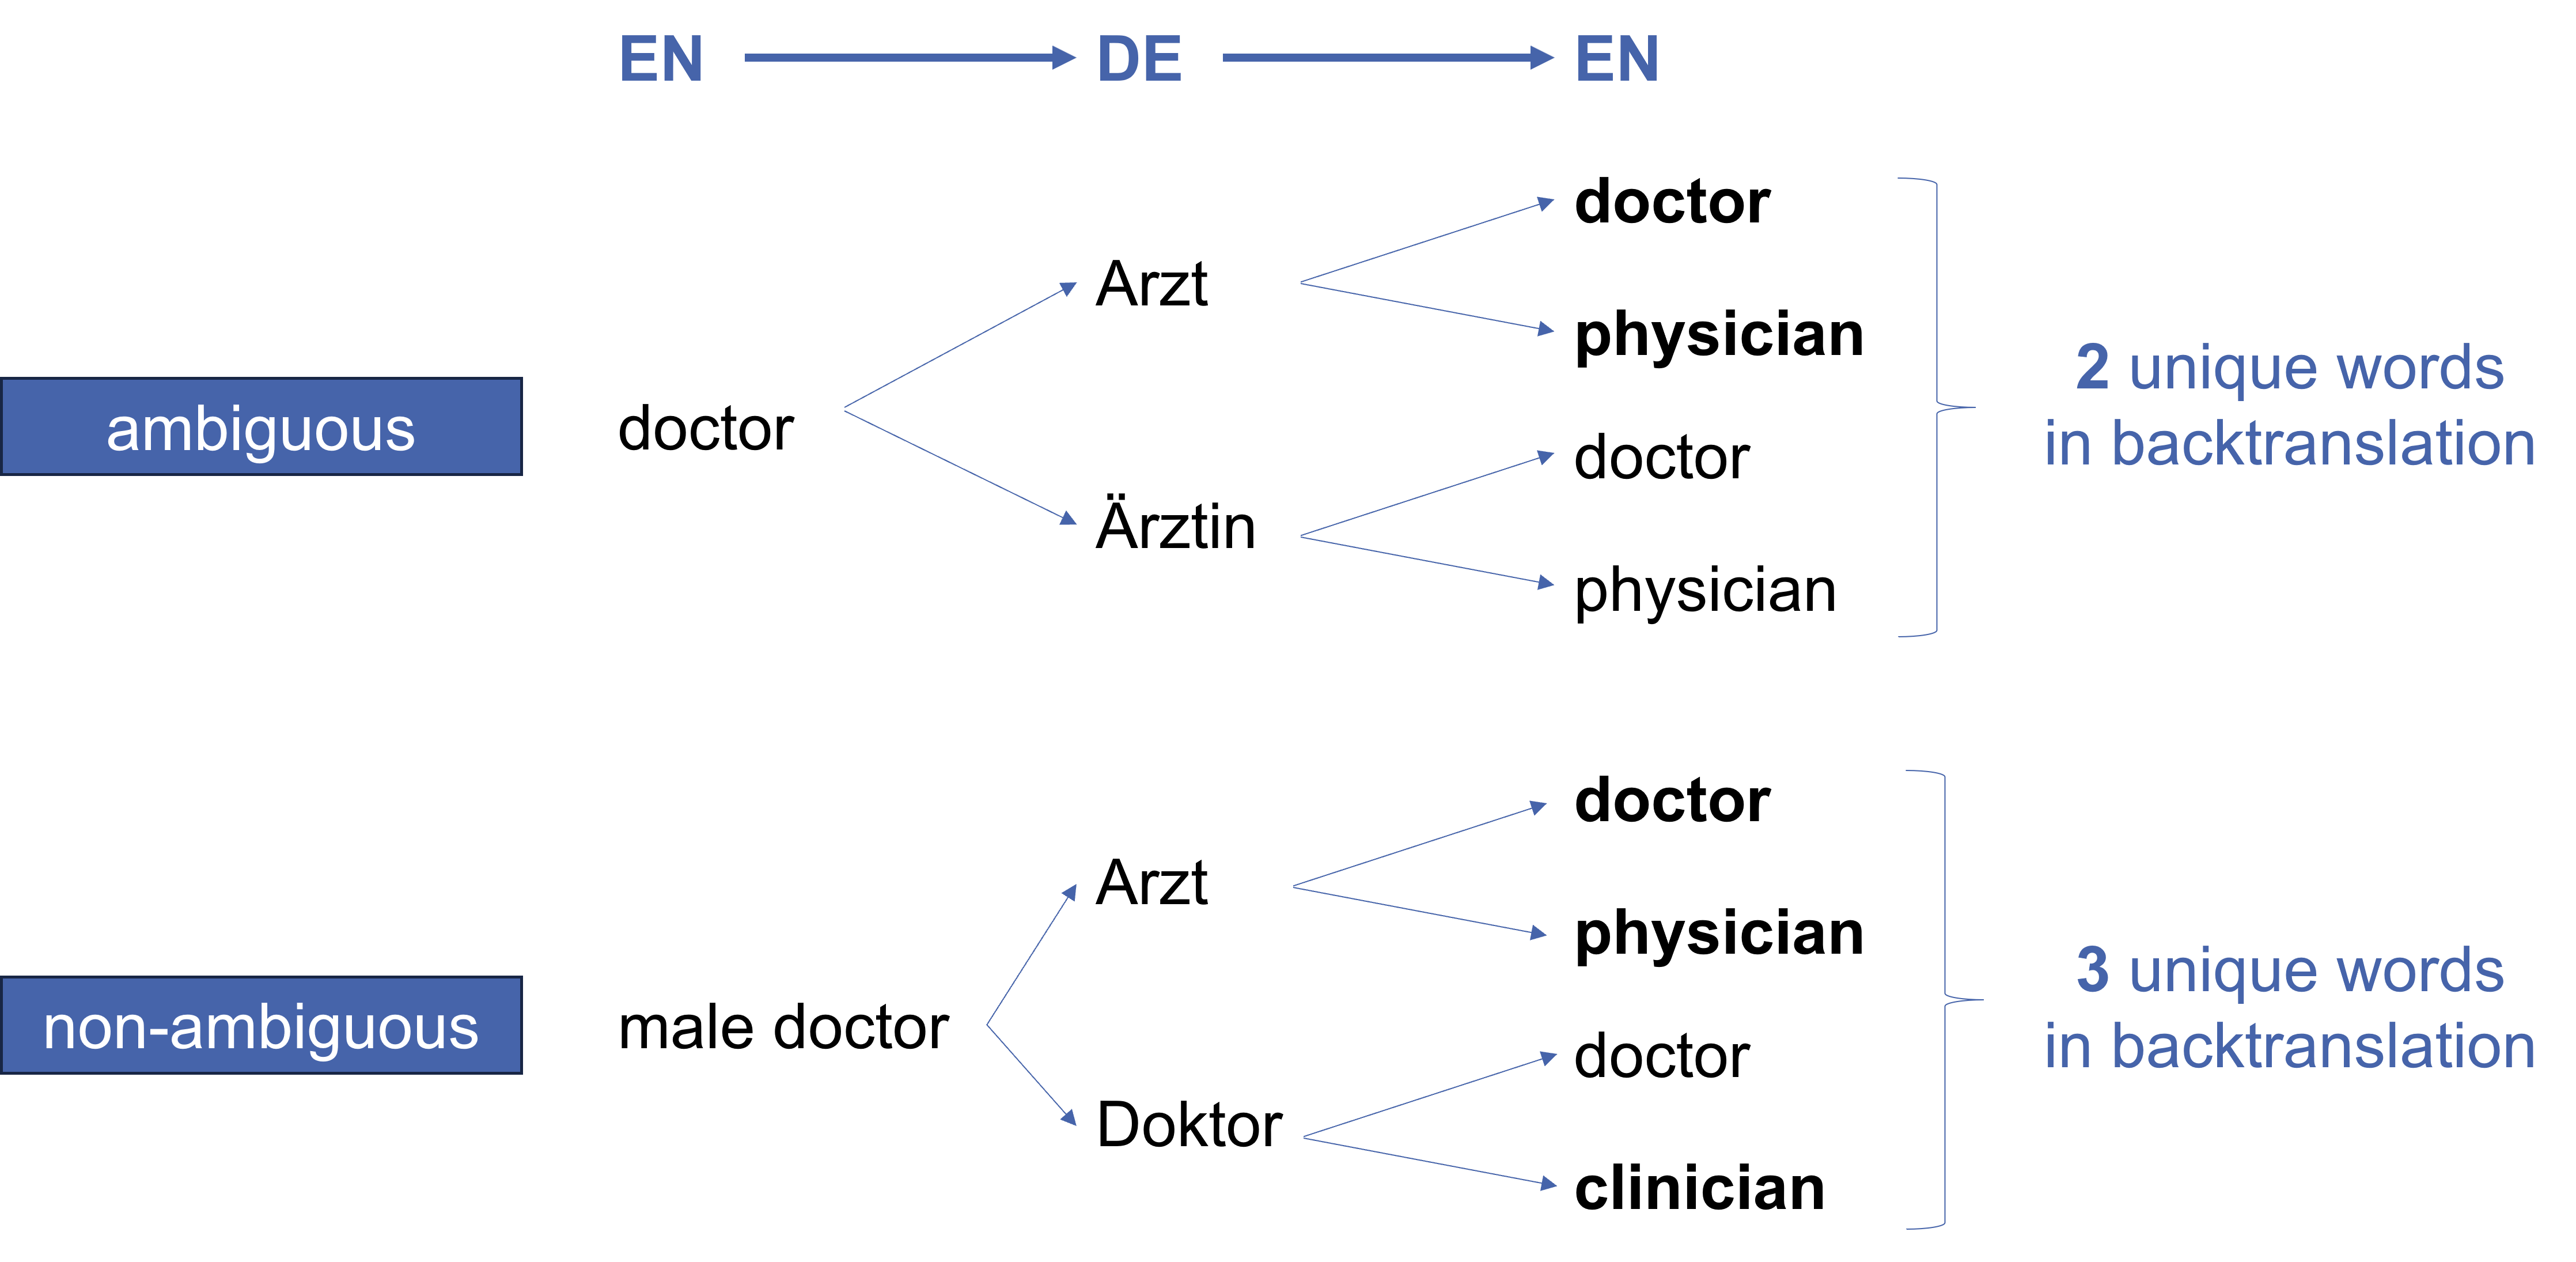
\includegraphics[scale=0.45]{figures/intuition.png}
  \caption{Example Illustration of the Intuition}
  \label{fig:intuition}
\end{figure}

Next, I will perform a more thorough explanation of the different experimental steps followed to inspect the assumption.



